\section{Conclusion}

\subsection{Free-Form Visualization}

\subsubsection{Test samples prediction}

A sample of successful tests predictions is displayed in Fig. \ref{fig:output420} with the predicted label and the true label shown in the title. 

\begin{center}
	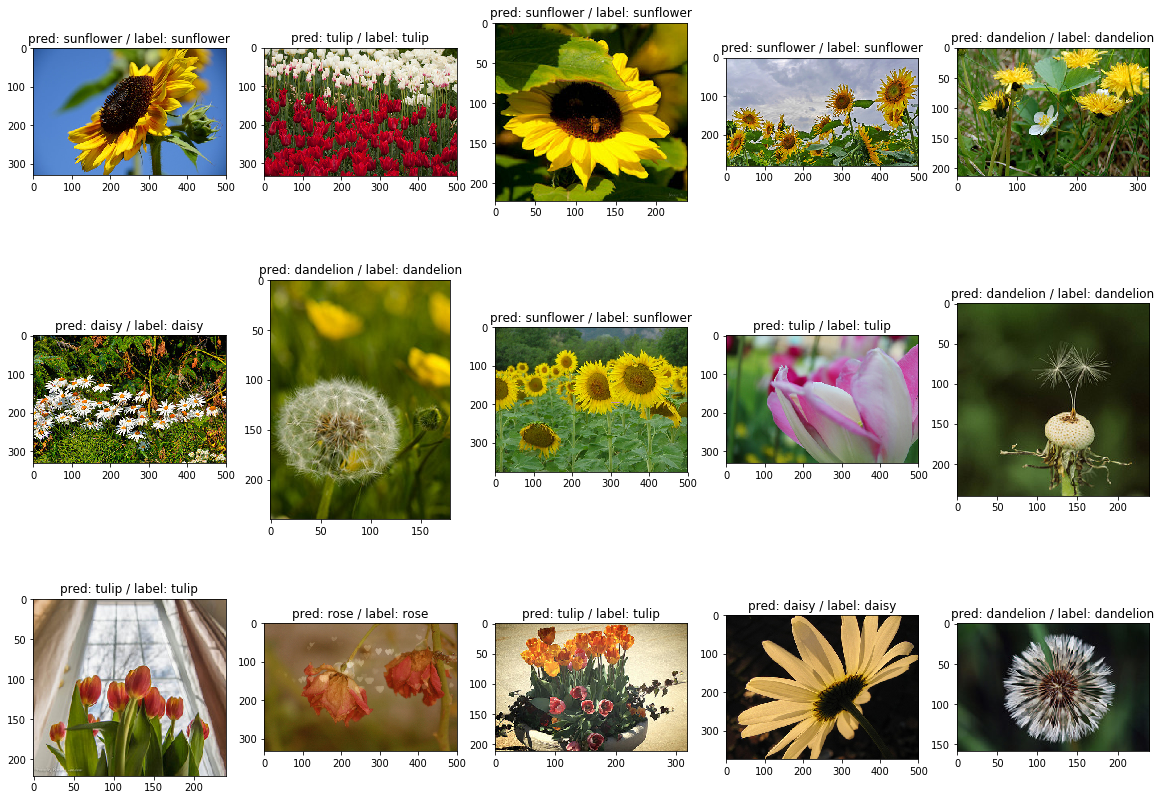
\includegraphics[scale=.35]{sections/05_conclusion/output_42_0}
	\captionof{figure}{Sample of test picture flower recognition}
	\label{fig:output420}
\end{center}

\subsubsection{Failed  prediction}

All the test samples that the model failed to identify correctly are display on Fig. \ref{fig:output430}.

\begin{center}
	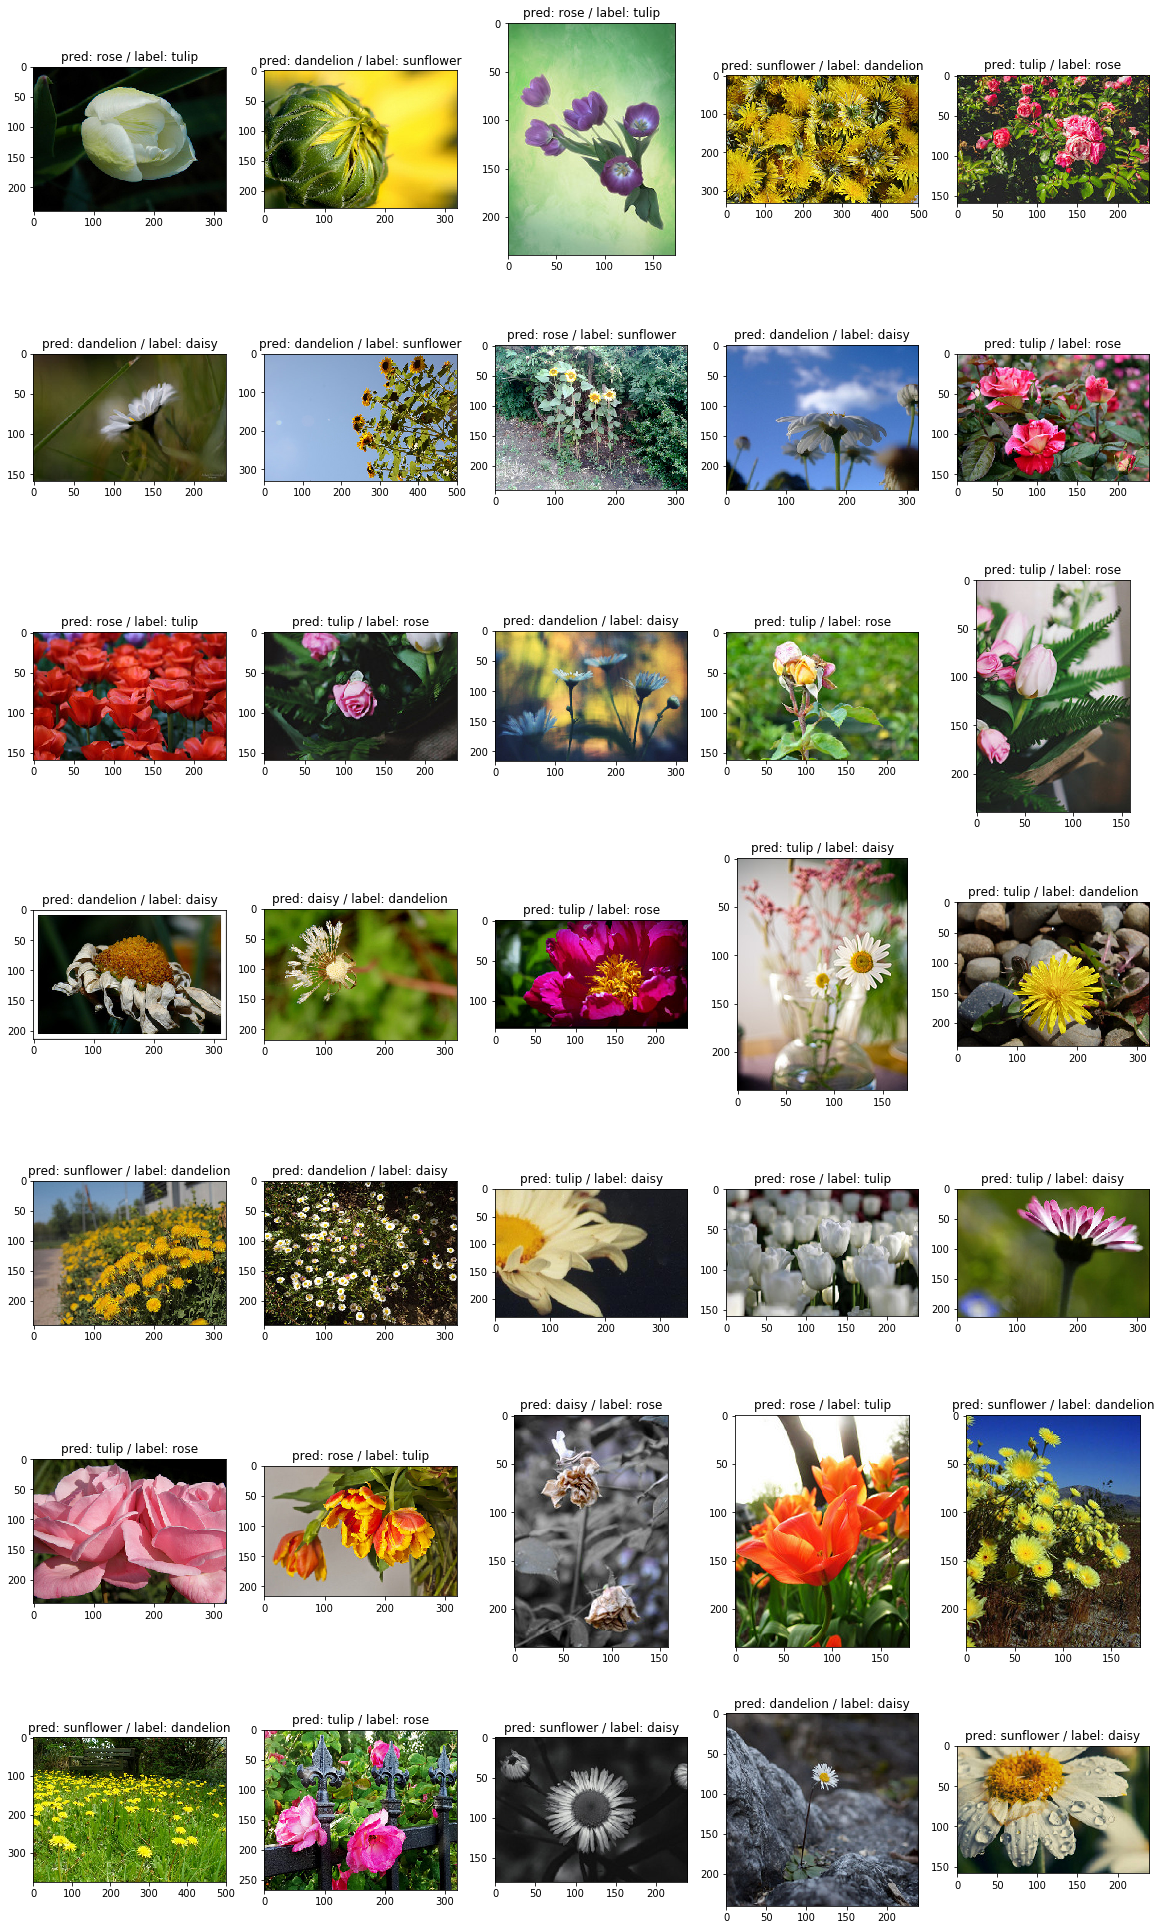
\includegraphics[scale=.35]{sections/05_conclusion/output_43_0}
	\captionof{figure}{failed predictions in the test dataset}
	\label{fig:output430}
\end{center}


\subsection{Reflection}

The process used for this project can be summarized as follow:

\begin{enumerate}
	\setlength\itemsep{1pt}
	\setlength{\parskip}{0pt}
	\setlength{\parsep}{0pt}
	\item Find a relevant/challenging problem to solve
	\item find already existing work(s) in order to set the benchmark
	\item Find a dataset suitable for answering this problem
	\item Clean up and pre-process the dataset to make it training-ready
	\item Test different base model for the CNN and select the best performing one
	\item Train the final chosen CNN in the cloud
	\item Evaluate the model and analyse the results
\end{enumerate}

One particular difficult and tedious task has been the manual selection of samples to keep or remove from the dataset. This work is hardly automatable and had to be performed case by case, based on arbitrary rules and intuition. 

I have been positively surprised by the differences in performance between the three based models tested. According to the references, VGG16 is the model among the three having the lowest accuracy on the ImageNet validation dataset \cite{Keras_applications}. However, this exercise comforted me in necessity to try different approaches.  

\subsection{Improvement}

The main improvement for this project would be to increase the amount of flower classes. It would be particularly interesting to train the same CNN on the 100+ flowers types used by the BiCos-SVM model \cite{Chai_BiCos_demo}.
It would also worth trying other base models that have not been considered in this study.
It would be beneficial to deeper analyse prediction failure cases in order to identify failures root cause and adapt accordingly the dataset or the model if feasible.
Finally, in order to deploy the model in real life, it would be necessary to develop a mobile application able to directly process a picture taken by the device and return to the user a prediction.